Des considérations géométriques classiques amènent à constater que le point de contacte $R$ est fait l'intersection d'une ellipse de foyers $S$ et $I$ qui est aussi tangente au cercle $\setgeo{C}$ : on utilise une propriété connue de rebond des ondes sur une ellipse utilisée dans certaines gares de métro
\footnote{
	Merci à mon collègue Jean-Marie B. de m'avoir rappelé cette \og évidence elliptique \fg\ .
}.

\begin{center}
	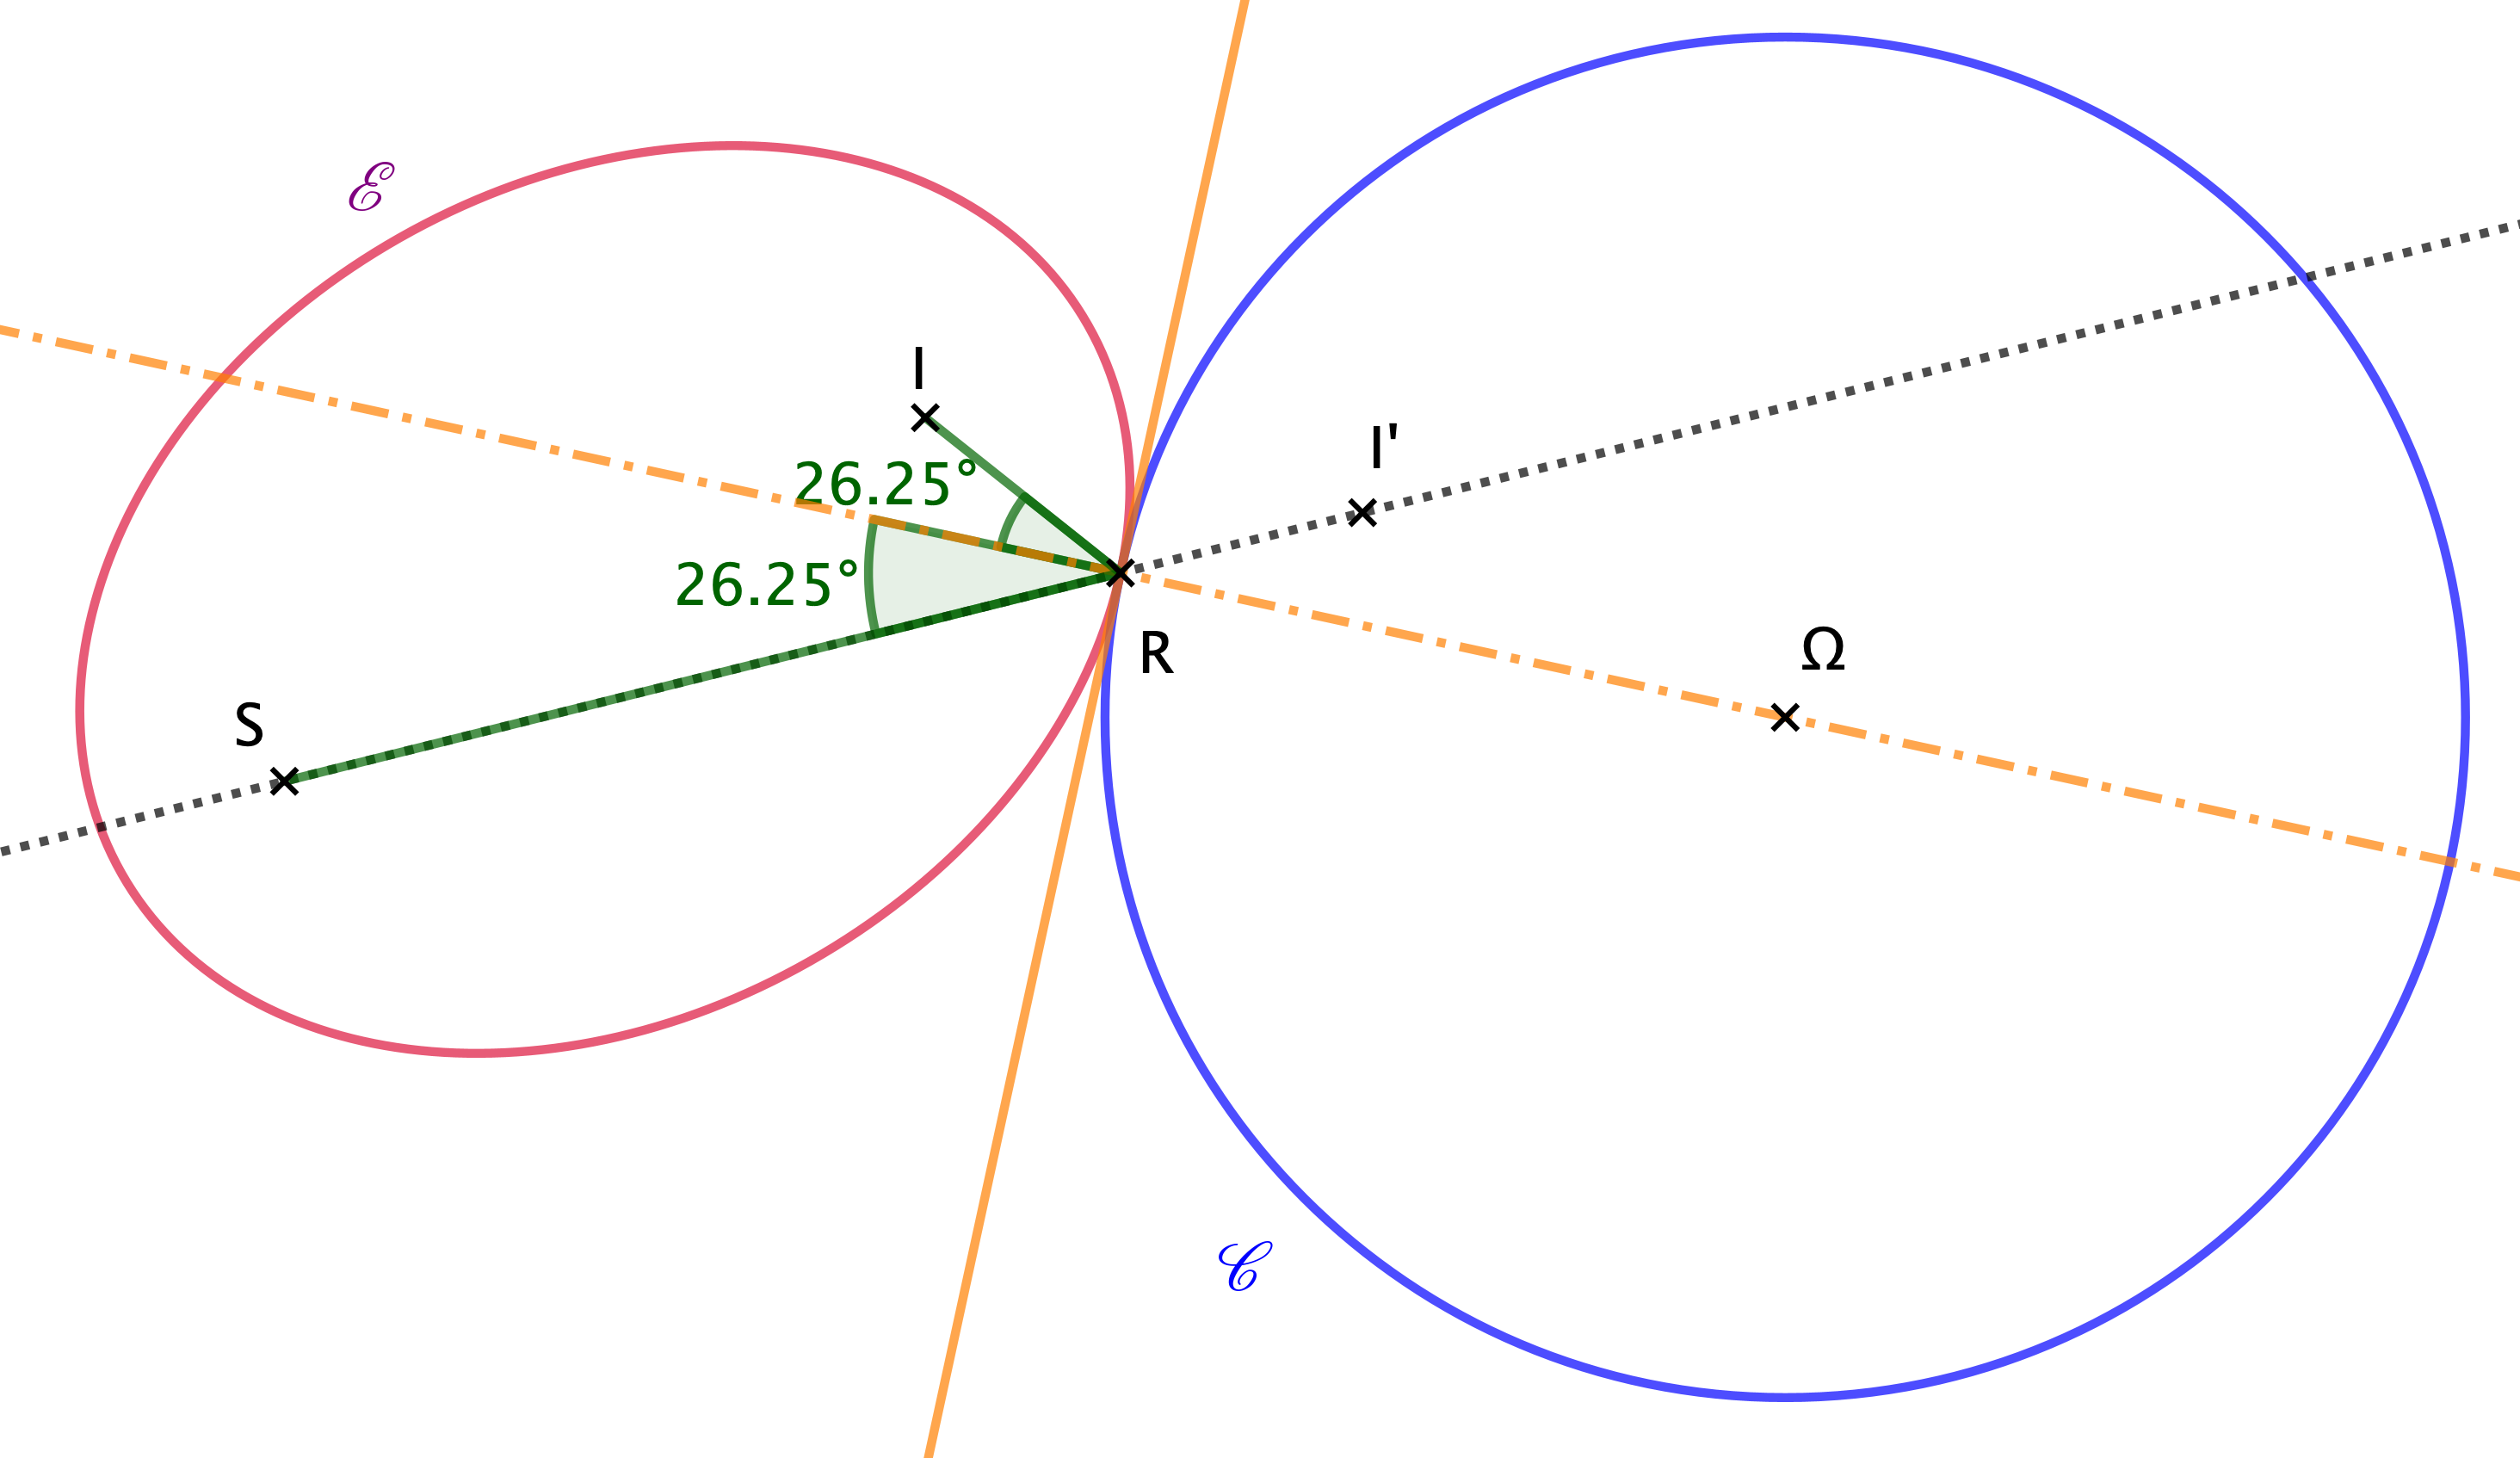
\includegraphics[scale=1.25]{ellipse.png}
\end{center}


Il reste à voir comment déterminer cette ellipse. Pour cela, on se place dans un repère orthonormé tel que l'on ait les faits suivantes.

\begin{itemize}[label=\small\textbullet]
	\item L'origine $O$ du repère est le milieu du segment $[SI]$ .

	\item $S\coord{1 | 0}$ et $I\coord{-1 | 0}$ .
\end{itemize}


Notant $\Omega\coord{p | q}$ , nous avons alors
$\setgeo{C} : (x - p)^2 + (y - q)^2 = r^2$
et
$\setgeo{E} : \dfrac{x^2}{a^2} + \dfrac{y^2}{b^2} = 1$ avec a minima $\coord{a | b | r} \in \big(\RRsp\big)^3$ .
On doit trouver $a$ et $b$ tels que $\card \big( \setgeo{C} \cap \setgeo{E} \big) = 1$ .


\bigskip


Nous avons pour $P\coord{x | y} \in \setgeo{C} \cap \setgeo{E}$ :

\medskip

\begin{stepcalc}[style=ar*, ope=\implies]
	(x - p)^2 + (y - q)^2 = r^2
\explnext*{$\rho = r^2$}{}
	x^2 - 2 p x + p^2 + y^2 - 2 q y + q^2 = \rho
%\end{stepcalc}
%
%\begin{stepcalc}[style=ar*, ope=\implies]
%	x^2 - 2 p x + p^2 + y^2 - 2 q y + q^2 = \rho
\explnext*{$\setgeo{E} : b^2 x^2 + a^2 y^2 = a^2 b^2$}{}
	a^2 x^2 - 2 p a^2 x + p^2 a^2 + (a^2 b^2 - b^2 x^2) - 2 q a^2 y + a^2 q^2 = a^2 \rho
\explnext*{$\alpha = a^2$ , $\beta = b^2$ , $\gamma = a^2 b^2$}{}
	\alpha x^2 - 2 p \alpha x + p^2 \alpha + (\gamma - \beta x^2) - 2 q \alpha y + \alpha q^2 = \alpha \rho
\explnext{}
      2 q \alpha y
    =
	  (\alpha - \beta) x^2 
	- 2 p \alpha x 
	+ \alpha(p^2 + q^2) 
	+ \gamma - \alpha \rho
\end{stepcalc}


\bigskip


Nous savons que $\alpha > 0$ , mais il est aussi immédiat que la configuration proposée empêche d'avoir $q = 0$ , nous avons ensuite :

\medskip

\begin{stepcalc}[style=ar*, ope=\implies]
	\beta x^2 + \alpha y^2 = \gamma
\explnext{}
    4 q^2 \alpha \beta x^2 + 4 q^2 \alpha^2 y^2 = 4 q^2 \alpha \gamma
\explnext{}
    4 q^2 \alpha \beta x^2 
    + 
    \big(
    	(\alpha - \beta) x^2 
	- 2 p \alpha x 
	+ \alpha(p^2 + q^2) 
	+ \gamma - \alpha \rho
    \big)^2
    =
    4 q^2 \alpha \gamma
\end{stepcalc}

